A body-fat scale sends a tiny alternating current through the feet and legs (you don't feel it). The water outside the cells conducts like a resistor $R_e$. The cells add a second path: the water inside them, a resistor $R_i$, behind their membranes, which act like a capacitor $C$. The graph shows the measured impedance against the frequency (logarithmic axis).

\begin{center}
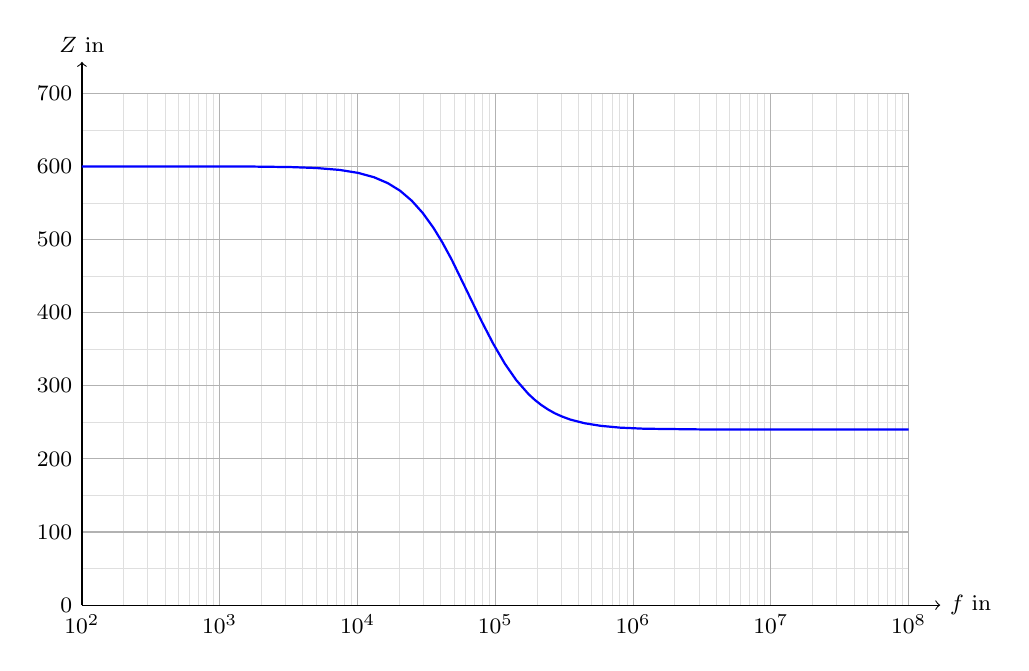
\begin{tikzpicture}[font=\footnotesize]
 \draw[gray!25, very thin] (0.527,0) -- (0.527,6.500) (0.835,0) -- (0.835,6.500) (1.054,0) -- (1.054,6.500) (1.223,0) -- (1.223,6.500) (1.362,0) -- (1.362,6.500) (1.479,0) -- (1.479,6.500) (1.580,0) -- (1.580,6.500) (1.670,0) -- (1.670,6.500) (2.277,0) -- (2.277,6.500) (2.585,0) -- (2.585,6.500) (2.804,0) -- (2.804,6.500) (2.973,0) -- (2.973,6.500) (3.112,0) -- (3.112,6.500) (3.229,0) -- (3.229,6.500) (3.330,0) -- (3.330,6.500) (3.420,0) -- (3.420,6.500) (4.027,0) -- (4.027,6.500) (4.335,0) -- (4.335,6.500) (4.554,0) -- (4.554,6.500) (4.723,0) -- (4.723,6.500) (4.862,0) -- (4.862,6.500) (4.979,0) -- (4.979,6.500) (5.080,0) -- (5.080,6.500) (5.170,0) -- (5.170,6.500) (5.777,0) -- (5.777,6.500) (6.085,0) -- (6.085,6.500) (6.304,0) -- (6.304,6.500) (6.473,0) -- (6.473,6.500) (6.612,0) -- (6.612,6.500) (6.729,0) -- (6.729,6.500) (6.830,0) -- (6.830,6.500) (6.920,0) -- (6.920,6.500) (7.527,0) -- (7.527,6.500) (7.835,0) -- (7.835,6.500) (8.054,0) -- (8.054,6.500) (8.223,0) -- (8.223,6.500) (8.362,0) -- (8.362,6.500) (8.479,0) -- (8.479,6.500) (8.580,0) -- (8.580,6.500) (8.670,0) -- (8.670,6.500) (9.277,0) -- (9.277,6.500) (9.585,0) -- (9.585,6.500) (9.804,0) -- (9.804,6.500) (9.973,0) -- (9.973,6.500) (10.112,0) -- (10.112,6.500) (10.229,0) -- (10.229,6.500) (10.330,0) -- (10.330,6.500) (10.420,0) -- (10.420,6.500);
 \draw[gray!25, very thin] (0,0.464) -- (10.500,0.464) (0,1.393) -- (10.500,1.393) (0,2.321) -- (10.500,2.321) (0,3.250) -- (10.500,3.250) (0,4.179) -- (10.500,4.179) (0,5.107) -- (10.500,5.107) (0,6.036) -- (10.500,6.036);
 \draw[gray!60, thin] (0.000,0) -- (0.000,6.500) (1.750,0) -- (1.750,6.500) (3.500,0) -- (3.500,6.500) (5.250,0) -- (5.250,6.500) (7.000,0) -- (7.000,6.500) (8.750,0) -- (8.750,6.500) (10.500,0) -- (10.500,6.500);
 \draw[gray!60, thin] (0,0.000) -- (10.500,0.000) (0,0.929) -- (10.500,0.929) (0,1.857) -- (10.500,1.857) (0,2.786) -- (10.500,2.786) (0,3.714) -- (10.500,3.714) (0,4.643) -- (10.500,4.643) (0,5.571) -- (10.500,5.571) (0,6.500) -- (10.500,6.500);
 \node[below] at (0.000,0) {$10^{2}$};
 \node[below] at (1.750,0) {$10^{3}$};
 \node[below] at (3.500,0) {$10^{4}$};
 \node[below] at (5.250,0) {$10^{5}$};
 \node[below] at (7.000,0) {$10^{6}$};
 \node[below] at (8.750,0) {$10^{7}$};
 \node[below] at (10.500,0) {$10^{8}$};
 \node[left] at (0,0.000) {0};
 \node[left] at (0,0.929) {100};
 \node[left] at (0,1.857) {200};
 \node[left] at (0,2.786) {300};
 \node[left] at (0,3.714) {400};
 \node[left] at (0,4.643) {500};
 \node[left] at (0,5.571) {600};
 \node[left] at (0,6.500) {700};
 \draw[->] (0,0) -- (10.900,0) node[right] {$f$ in \si{\hertz}};
 \draw[->] (0,0) -- (0,6.900) node[above] {$Z$ in \si{\ohm}};
 \draw[thick, blue] plot coordinates {(0.000,5.571) (2.193,5.569) (2.650,5.563) (2.977,5.551) (3.271,5.527) (3.508,5.489) (3.709,5.434) (3.884,5.359) (4.041,5.262) (4.188,5.136) (4.328,4.980) (4.465,4.790) (4.577,4.606) (4.698,4.383) (5.079,3.598) (5.225,3.316) (5.372,3.064) (5.515,2.858) (5.669,2.682) (5.750,2.607) (5.832,2.542) (5.918,2.485) (6.007,2.435) (6.102,2.393) (6.203,2.356) (6.382,2.310) (6.586,2.277) (6.831,2.254) (7.141,2.240) (7.971,2.230) (10.500,2.229)};
\end{tikzpicture}
\end{center}

\begin{abcliste}
\abc What is $R_e$?
\abc What is $R_i$?
\abc Most scales measure at \SI{50}{\kilo\hertz}. Which impedance do they see?
\end{abcliste}
